%%% template.tex
%%%
%%% This LaTeX source document can be used as the basis for your technical
%%% paper or abstract. Regardless of the length of your document, the commands
%%% are all the same.
%%% 
%%% The "\documentclass" command is the first command in your file. If you want to 
%%% prepare a version of your article with line numbers - a "review" version - 
%%% include the "review" parameter:
%%%    \documentclass[review]{acmsiggraph}
%%%
%%%[annual/preprint/review]
\documentclass[review]{acmsiggraph}

\usepackage{amsmath,amssymb}
\usepackage{xcolor}
\usepackage{algorithm,algorithmic}
\usepackage{overpic}
\usepackage{todonotes}
\usepackage{tabularx}
\usepackage{tikz}
\usepackage{subfig}
\usepackage{xcolor,colortbl}

\title{Linear Time Optimization}

\author{LIRIS}
\pdfauthor{LIRIS}

\TOGonlineid{0015}

\keywords{Monte Carlo and Quasi-Monte Carlo Integration, Sampling, Variance Reduction, Anti-Aliasing, Rendering}

\graphicspath{{./figures/}}

% With the "\setcopyright" command the appropriate rights management text will be added
% to your document.

%\setcopyright{none}
%\setcopyright{acmcopyright}
%\setcopyright{acmlicensed}
\setcopyright{rightsretained}
%\setcopyright{usgov}
%\setcopyright{usgovmixed}
%\setcopyright{cagov}
%\setcopyright{cagovmixed}
%\setcopyright{rightsretained}

% The year of publication in the "\copyrightyear" command.

%\copyrightyear{2016}

%%% Conference information, from the completed rights management form.
%%% The "\conferenceinfo" command has two parameters: 
%%%    - conference name
%%%    - conference date and location
%%% The "\isbn" field includes the year and month after the article ISBN.

%\conferenceinfo{SIGGRAPH 2016 Posters}{July 24-28, 2016, Anaheim, CA} 
%\isbn{978-1-4503-ABCD-E/16/07} 
%\doi{http://doi.acm.org/10.1145/9999997.9999999}

\begin{document}

\include{macros}

%%% This is the ``teaser'' command, which puts an figure, centered, below 
%%% the title and author information, and above the body of the content.
%
% \teaser{
%   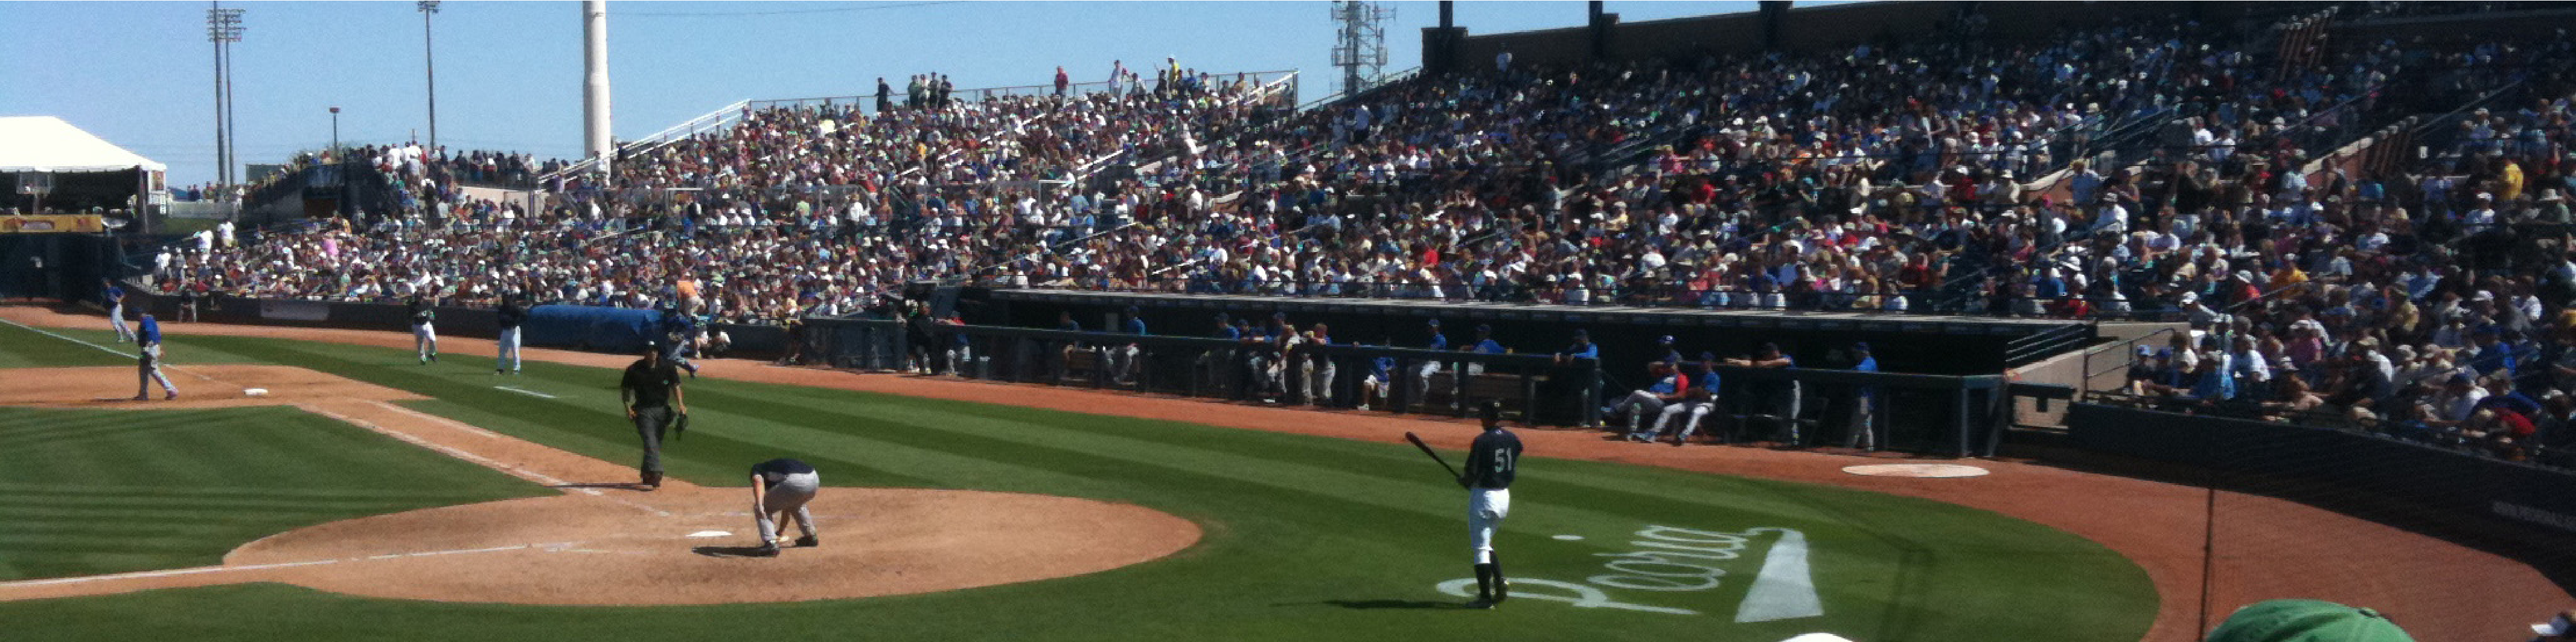
\includegraphics[height=1.5in]{images/sampleteaser}
%   \caption{Spring Training 2009, Peoria, AZ.}
% }

\maketitle

%%%%%%%%%%%%%%%%%%%%%%%%%%%%%%%%%%%%%%%%%%%%%%%%%%%%%%%%%%%%%%%%%%%%%%%%%%%%%%%%%%%%%%
%%% Abstract
%%%%%%%%%%%%%%%%%%%%%%%%%%%%%%%%%%%%%%%%%%%%%%%%%%%%%%%%%%%%%%%%%%%%%%%%%%%%%%%%%%%%%%

\begin{abstract}

Distributions of samples play very important role in rendering,
\end{abstract}

\begin{CCSXML}
<ccs2012>
<concept>
<concept_id>10010147.10010371.10010372</concept_id>
<concept_desc>Computing methodologies~Rendering</concept_desc>
<concept_significance>500</concept_significance>
</concept>
</ccs2012>
\end{CCSXML}
\ccsdesc[500]{Computing methodologies~Rendering}

\keywordlist

\conceptlist

%\printcopyright

%%%%%%%%%%%%%%%%%%%%%%%%%%%%%%%%%%%%%%%%%%%%%%%%%%%%%%%%%%%%%%%%%%%%%%%%%%%%%%%%%%%%%%
%%% Motivation
%%%%%%%%%%%%%%%%%%%%%%%%%%%%%%%%%%%%%%%%%%%%%%%%%%%%%%%%%%%%%%%%%%%%%%%%%%%%%%%%%%%%%%

\section{Motivation}
\label{sec:Motivation}

Monte Carlo and Quasi-Monte-Carlo (MCQMC) integration is widely used
to evaluate the rendering equation~\cite{Pharr2016}, where
Low-discrepancy sequences (LDS) play a crucial
role~\cite{Niederreiter1992,Lemieux2009}, because of their inherent
virtues: guaranteed hight degree of uniformity, computational
efficiency, easy and compact implementation.



\bibliographystyle{acmsiggraph}
\bibliography{LinearTimeOptimization}
\end{document}
